\section{Introduction}
%
In this project, we aim to establish a scope which covers two fields: \emph{robotics} and \emph{deep learning}.\\

In the last decades, robots have become a powerful allied to humans, as they are leveraged to perform all kind of tasks (hazardous explorations, personal assistance, cleaning, driving, \dots). However, we aim to design them to perform these tasks on the most autonomous way possible, which means not requiring to be controlled on every action (with exceptions, such as surgeon robots). This requires to provide robots a certain intelligence and capabilities to correctly trigger the most suitable action for each possible input stimulus. For this purpose, we can find multiple approaches for different problems (navigation, conversation, \dots).\\

We will focus in the \emph{Computer Vision} field, which involves connecting cameras to a robot, and taking advantage of this on an autonomous way. Concretely, we will tackle the person following challenge, which is based on a behavior governed by a \emph{person detection} system. Many approaches are already existing, such as color filters, or disparities filtering. However, promising \emph{Deep Learning} techniques excel on their image processing variant, as it offers high quality results, accompanied by \emph{robustness} facing lighting issues (Fig. \ref{fig:intro_harsh_light}). This is the set of techniques we have used on this project, so we will describe the basis firstly.\\

\begin{figure}[h]
	\centering
	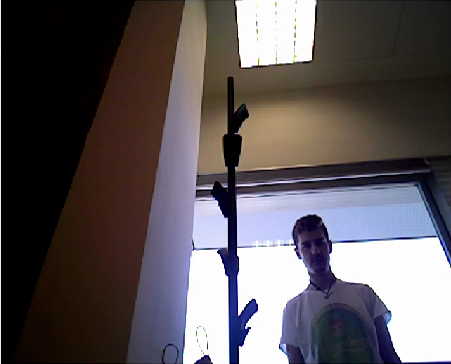
\includegraphics[width=2in]{images/light_ko_2}
	\caption{Harsh lighting situation for \emph{Computer Vision} algorithms.}
	\label{fig:intro_harsh_light}
\end{figure}


\subsection{Artificial Neural Networks (\emph{ANNs})}


A Neural Network is the representation of an algebraic algorithm which implements non-linear calculus models [10 en tfg]. It is composed by successive processing \emph{layers}, which are made up of \emph{perceptrons} (generally called \emph{neurons}). This is because these neural structures \emph{emulate the human brain}, formed by a huge set of interconnected neurons, which are disposed on the already mentioned layers (Fig. \ref{fig:intro_neural_network})


\begin{figure}[h]
	\centering
	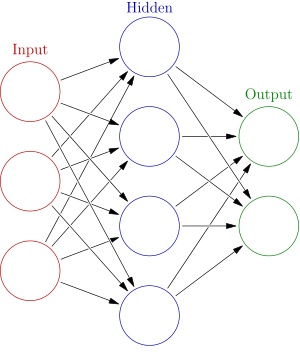
\includegraphics[width=1.5in]{images/neural_network}
	\caption{Structure of a Neural Network}
	\label{fig:intro_neural_network}
\end{figure}


\subsection{Processing unit: the perceptron (neuron)}


\subsection{Deep Neural Networks}


\subsection{Convolutional Neural Networks}



















\subsection{kaka}

In the image detection quandary, we aim to determine \emph{presence and position} of a certain object in a given image. For this, we will make use of \emph{deep neural networks}, which are processing structures which try to emulate a biological brain.\\


\begin{figure}[h]
	\centering
	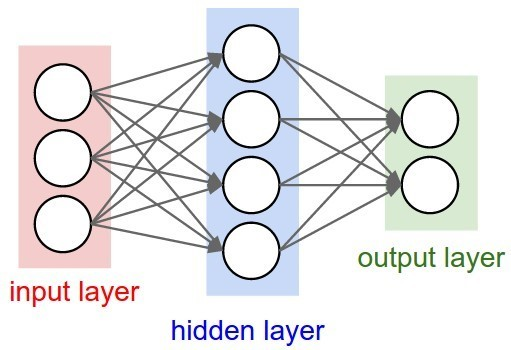
\includegraphics[width=2.5in]{images/neural_network_2}
	\caption{Neural Network.}
\end{figure}


They are composed by \emph{perceptrons} (what are called \emph{neurons}). These perceptrons implement an internal pipeline, which is applied to its input, what we call the \emph{activation region}.


%\textsl{}